%------------------------------------------------------------------------------%
%                                   hedgehog                                   %
%------------------------------------------------------------------------------%

\section{Hedgehog}
\label{sec:hh}

\gls{hh} is a template library designed to create parallel implementations using
data-flow graphs. It is the direct successor of \gls{hmbe}, which also utilized
data-flow graphs \cite{blattner2017model}. \gls{hh} was developed as part of
Alexandre Bardakoff's PhD thesis at NIST \cite{bardakoff2021analysis}.

In this section, we will present some of the features of the library and how
we can use it to express an algorithm under the form of a graph.

\subsection{The data-flow graphs}

As mentioned in the introduction of this section, algorithms are expressed as
data-flow graphs. A data-flow graph is a graphical representation where edges
denote data streams and vertices represent tasks as explained by
\cite{kavi1986formal} and \cite{bardakoff2021analysis}. An example of a
data-flow graph is shown in Figure \ref{fig:data-flow-graph-example}.

% [Data-flow graph example] {{{
\begin{figure}[h!]
  \begin{center}
    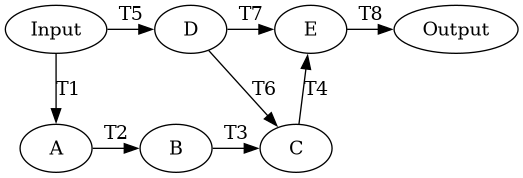
\includegraphics[scale=0.5]{./img/data-flow-graph-example.png}
    \caption{Data-flow graph example}
    \label{fig:data-flow-graph-example}
  \end{center}
\end{figure}
%}}}

In each task, the input data is consumed and transformed into new data that
serves as input to other tasks. For instance, in Figure
\ref{fig:data-flow-graph-example}, there are two inputs of types \texttt{T1} and
\texttt{T5}. The data of type \texttt{T1} is input into Task \texttt{A} that
produces new data of type \texttt{T2} that is transmitted to Task \texttt{B}.
At the end of the graph, Task \texttt{E} generates data of type \texttt{T8}
that is the output of the graph.

In \gls{hh}, the data are transmitted between nodes using shared pointers to
ensure efficiency even, with large data types.

\subsection{The nodes}

To design an algorithm using Hedgehog, we create a graph in which the data will
flow through various nodes. These nodes can be of different types, which we
describe in this section.

\subsubsection{Tasks}

The first type of nodes are the tasks. These nodes are made to be duplicated and
run in multiple threads. As all other nodes, a task can have multiple input and
output types.

On Listing \ref{lst:hhtask}, we can see how to create a task using \gls{hh}.
To do this, we define a class that inherits from \texttt{hh::AbstractTask} and
we override the \texttt{execute} and \texttt{copy} functions. The
\texttt{execute} functions are called when the task receives a data of a certain
type and the \texttt{copy} function is used to duplicate the task to run on
multiple threads.

The tasks have at least three template parameters. The first one is the number
of input types (in this example, we have two input types) and it is followed by
the list of the input types (T3 and T6) and the list of the output types (T4).

%- begin listing ------------------------------------------------------------{{{
\begin{listing}[ht!]
\begin{minted}[frame=lines,framesep=2mm,baselinestretch=1.2,fontsize=\normalsize,linenos]{C++}
  class C: public hh::AbstractTask<2, T6, T3, T4> {
  public:
    SubLineTask(size_t nbThreads):
        hh::AbstractTask<2, T6, T3, T4>("C", nbThreads) {}

    void execute(std::shared_ptr<T3> data) override {
      // compute with T3 data
      return std::make_shared<T4>(/* ... */)
    }

    void execute(std::shared_ptr<T6> data) override {
      // compute with T6 data
      return std::make_shared<T4>(/* ... */)
    }

    std::shared_ptr<hh::AbstractTask<2, T6, T3, T4>>
    copy() override {
        return std::make_shared<C>(this->numberThreads());
    }
};
\end{minted}
\captionof{listing}{Hedgehog: Task}
\label{lst:hhtask}
\end{listing}
%- end listing --------------------------------------------------------------}}}

\subsubsection{States}

States are special nodes used only for synchronisation and cannot be duplicated.
They are thread-safe and control the data-flow in the graph. It is important to
be careful when creating a state as it locks the program using a mutex. This
means that only simple operations have to be made in the states in order not to
slow the program execution.

Creating a state is very similar to creating a task. A state inherits from
\texttt{hh::AbstractState} and overrides the \texttt{execute} function. However,
states do not have a \texttt{copy} function, as they should not be parallelized.

A state cannot be used directly in a graph and must be managed by a state
manager, which is described in Section \ref{sec:statemanager}.

\subsubsection{State Managers}
\label{sec:statemanager}

A state manager is a node that owns a state. It handles locking the state when
data is received. Multiple state managers can own the same state in a graph,
which allows reuse of the state at different stages of the computation. \gls{hh}
provides a default implementation for the state manager, but users can create
custom ones to handle cycles.

One of the key features of \gls{hh} is the fact that it allows the creation of
cycles in the graphs. This is particularly useful for repeating operations
(loops in computation). However, it is not possible to automatically detect when
a cycle can be broken at runtime. Users can implement their own state managers
and override the \texttt{canTerminate} function to control when a state should
stop.

Listing \ref{lst:statemanager} provides an example of a state manager for a type
\texttt{MyState}. Here, the \texttt{canTerminate} function is overridden to
return whether the state is finished. In this function, the state is locked, and
the \texttt{isDone} method (defined in the state) is used to know if the state
can be finished. The template parameters of the \texttt{StateManager} should
match the parameters used when creating the state.

%- begin listing ------------------------------------------------------------{{{
\begin{listing}[ht!]
\begin{minted}[frame=lines,framesep=2mm,baselinestretch=1.2,fontsize=\normalsize,linenos]{C++}
  class MySM: public hh::StateManager<1, T1, T2, T3, T4> {
  public:
    MySM(std::shared_ptr<MyState> const& state):
        hh::StateManager<1, T1, T2, T3, T4>(state, "My SM") { }

    [[nodiscard]] bool canTerminate() const override {
        this->state()->lock();
        auto ret = std::dynamic_pointer_cast<MyState>(this->state())->isDone();
        this->state()->unlock();
        return ret;
    }
};
\end{minted}
\captionof{listing}{Hedgehog: state manager}
\label{lst:statemanager}
\end{listing}
%- end listing --------------------------------------------------------------}}}

\subsubsection{Graphs}

Graphs themselves are nodes as well, meaning that a graph can contain other
graphs. In a graph, nodes are connected by edges in order for them to be able to
communicate.

Listing \ref{lst:graph} shows how to create a graph. In this example, some nodes
are created (tasks and states), and the edges are defined to connect these
nodes. For instance, at Line 12, an edge between \texttt{myTask1} and
\texttt{myTask2} is created, meaning that the task one (the sender) will output
data to the task two (the receiver). To create an edge between two nodes, they
must share at least one type (if task one outputs a data of type \texttt{T1},
the task two should accept this type as input). Like other nodes, graphs have
inputs and outputs, which can be specified using the corresponding methods.
\clearpage{}

%- begin listing ------------------------------------------------------------{{{
\begin{listing}[ht!]
\begin{minted}[frame=lines,framesep=2mm,baselinestretch=1.2,fontsize=\normalsize,linenos]{C++}
class MyGraph: public hh::Graph<1, T1, T2> {
  public:
    GaussGraph(size_t matrixHeight, size_t nbThreads):
        hh::Graph<1, T1, T2>("My Graph") {
      auto myTask1 = std::make_shared<MyTask1>(/* nbThreads, ... */);
      auto myTask2 = std::make_shared<MyTask2>(/* nbThreads, ... */);
      auto myState = std::make_shared<MySate>(/* ... */);
      auto myStateManager = std::make_shared<MySM>(myState);

      this->inputs(myTask1);
      this->edges(mayTask1, myTaks2);
      this->edges(mayTask1, myStateManager);
      this->edges(mayTask2, myStateManager);
      this->edges(myStateManager, mayTask2);
      this->outputs(myStateManager);
    }
};
\end{minted}
\captionof{listing}{Hedgehog: graph}
\label{lst:graph}
\end{listing}
%- end listing --------------------------------------------------------------}}}

The graph class can be instantiated to create a graph to which data can be
pushed as shown in Listing \ref{lst:graphusage}. After pushing the data, the
function \texttt{finishPushingData} is called to start the computation, and
\texttt{waitForTermination} is used to wait for the end of the computation.

%- begin listing ------------------------------------------------------------{{{
\begin{listing}[ht!]
\begin{minted}[frame=lines,framesep=2mm,baselinestretch=1.2,fontsize=\normalsize,linenos]{C++}
MyGraph myGraph;

myGraph.executeGraph();
myGraph.pushData(/* ... */);
myGraph.finishPushingData();
myGraph.waitForTermination();
\end{minted}
\caption{Hedgehog: using a graph}
\label{lst:graphusage}
\end{listing}
%- end listing --------------------------------------------------------------}}}

\subsection{Profiling}

\gls{hh} includes a powerful profiling tool that generates a \textit{dot} file.
This file can be compiled using \textit{graphviz} \cite{graphviz} to generate an
image representing the graph. The generated graph contains detailed information
on the execution of the graph such as the execution time, the size of the
queues, the number of threads, and more. This information can be used to
optimize the graph by balancing the number threads between the tasks or
optimizing the tasks that are slower. It can also be used to refactor the
algorithm as it is very easy to identify the critical path on the image.

An example of a compiled dot file for a graph performing the Hadamar product
on two matrices is shown in Figure \ref{fig:tuto1}. This example is
presented in the tutorials in the \gls{hh}'s documentation \cite{hh:tuto}.

% [Output of the profiling tool (Hadamar Product)] {{{
\begin{figure}[h!]
  \begin{center}
    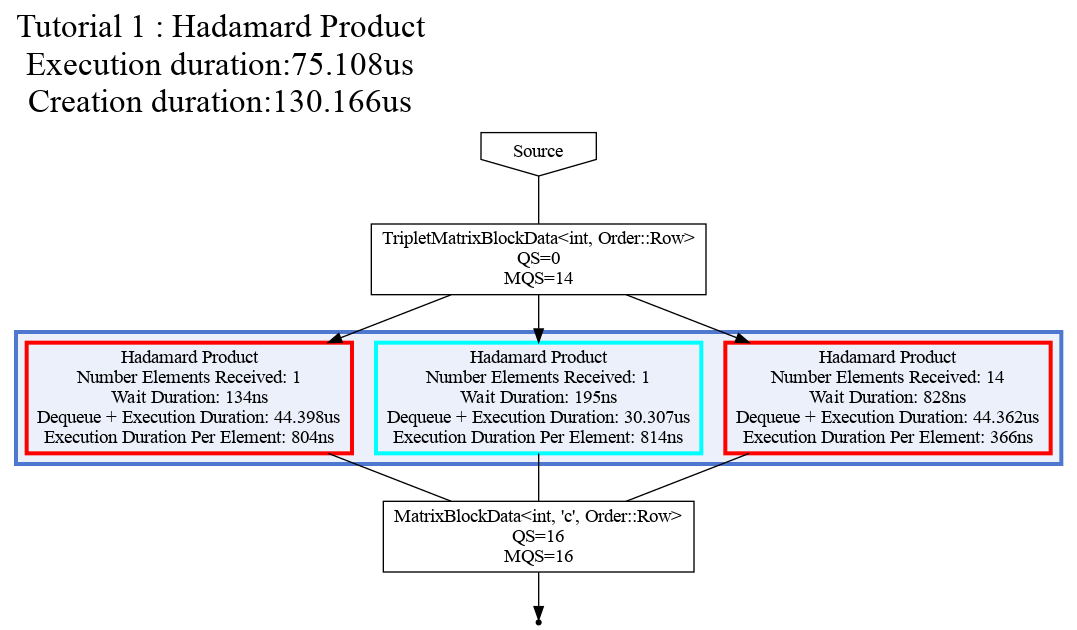
\includegraphics[scale=0.4]{img/Tutorial1HadamardProduct.png}
    \caption{Output of the profiling tool (Hadamar Product)}
    \label{fig:tuto1}
  \end{center}
\end{figure}
%}}}

It is important to note that the profiling tool is always active and incurs
minimal additional cost to the execution time of the graph
\cite{bardakoff2021analysis}.
